% Chapter 7 preview; compile from latex/.
\documentclass[11pt,a4paper]{report}
\usepackage[utf8]{inputenc}
\usepackage[T1]{fontenc}
\usepackage{lmodern}
\usepackage[provide=*,ngerman]{babel}
\usepackage[margin=25mm]{geometry}
\usepackage{amsmath,graphicx,booktabs,listings}
\usepackage{xurl}
\usepackage[hidelinks]{hyperref}
\graphicspath{{pictures/}}
\pdfminorversion=7
\lstset{literate={ö}{{\"o}}1 {ä}{{\"a}}1 {ü}{{\"u}}1
 {Ö}{{\"O}}1 {Ä}{{\"A}}1 {Ü}{{\"U}}1 {ß}{{\ss}}1}
\begin{document}
\setcounter{chapter}{6}
% !TeX root = ../main.tex

%%
%% Berliner Hochschule für Technik --  Abschlussarbeit
%%
%% Kapitel 7
%%
%%

\chapter{Auswertung der Berichte}
\section{Explorative Auswertung der Testable-Erhebung}
\label{sec:testable-auswertung}
% Generated by analyse_testable.R; do not edit numbers manually.
\newcommand{\TestableN}{66}
\newcommand{\TestableM}{61,42}
\newcommand{\TestableL}{60,81}
\newcommand{\TestableSDM}{17,52}
\newcommand{\TestableSDL}{16,88}
\newcommand{\TestableDiff}{-0,61}
\newcommand{\TestableSDDiff}{5,24}
\newcommand{\TestableLower}{-1,90}
\newcommand{\TestableUpper}{0,68}
\newcommand{\TestableT}{-0,948}
\newcommand{\TestableP}{0,173}
\newcommand{\TestableDz}{-0,117}
\newcommand{\TestableWilcoxonP}{0,678}
\newcommand{\TestableWilcoxonV}{977,5}
\newcommand{\TestableBootLo}{-1,90}
\newcommand{\TestableBootHi}{0,62}
\newcommand{\TestableAge}{40,95}
\newcommand{\TestableSDAge}{8,52}
\newcommand{\TestableCigs}{13,85}
\newcommand{\TestableSDCigs}{3,78}
\newcommand{\TestableDuration}{117,87}
\newcommand{\TestableDurationQone}{114,61}
\newcommand{\TestableDurationQthree}{132,38}



\subsection{Analysestichprobe und Datenqualität}

Von den 68 Ergebnisdateien der Testable-Studie besitzt eine keine Teilnehmerkennung, da sie aus einem Testlauf stammt, und eine andere Sitzung einen zusätzlichen Craving-Wert. Diese Ergebnisse gehen nicht in die Analyse ein. Die Analyse umfasst daher \TestableN{} Personen mit jeweils zwanzig eindeutig zugeordneten und gültigen Berichten und insgesamt 1320 Messwerten. Alle erfüllen die im Trial-File implementierten Screening-Grenzen von mindestens 30 Jahren und mindestens zehn Zigaretten pro Tag. Das mittlere Alter der Teilnehmenden beträgt \TestableAge{} Jahre (Spannweite 30--67), die angegebene tägliche Zigarettenzahl im Mittel \TestableCigs{} (Spannweite 10--25).

\subsection{Statistisches Vorgehen}
Die Berechnungen werden mit R 4.3.3 und den mitgelieferten Paketen durchgeführt.

Für jede Person $i$ werden zunächst die zehn Matching- und zehn Labeling-Werte gemittelt. Der zentrale Kontrast ist
\begin{equation}
 D_i=\overline{Y}_{i,L}-\overline{Y}_{i,M},\qquad
 \widehat{\Delta}=\frac{1}{n}\sum_{i=1}^{n}D_i.
\end{equation}
Negative Werte bedeuten geringeres Rauchverlangen nach Labeling. Jede Person erhält dasselbe Gewicht. Die 1320 Einzelberichte werden nicht als unabhängige Beobachtungen behandelt. Der Ein-Stichproben-$t$-Test der Personendifferenzen gegen null ist rechnerisch identisch mit einem gepaarten $t$-Test der beiden Personenmittelwerte. Berichtet werden außerdem die Standardabweichung $s_D$, das Intervall
\begin{equation}
 \widehat{\Delta}\ \pm\ t_{n-1;0{,}975}\frac{s_D}{\sqrt{n}}
 \quad\text{und}\quad d_z=\frac{\widehat{\Delta}}{s_D}.
\end{equation}

\subsection{Ergebnisse}
Die personenbezogenen Mittelwerte des Rauchverlangens betragen nach Matching \TestableM{} Punkte (SD \TestableSDM{}) und nach Labeling \TestableL{} Punkte (SD \TestableSDL{}). Die mittlere Differenz Labeling minus Matching ist \TestableDiff{} Punkte (SD der Differenzen \TestableSDDiff{}; 95\,\%-KI [\TestableLower{}; \TestableUpper{}]). Der gepaarte Vergleich ergibt $t(65)=\TestableT$, $p=\TestableP$ und $d_z=\TestableDz$. Damit liefern die Daten keinen statistisch belastbaren Nachweis eines mittleren Unterschieds zwischen den Bedingungen in diesem Ablauf.

Bei 32 Personen ist der Mittelwert nach Labeling niedriger, bei 32 höher. rei zwei Personen sind beide Mittelwerte gleich. Der Median der Personendifferenzen beträgt null. Abbildung \ref{fig:testable-paired} zeigt die Personendifferenzen. Null ist gestrichelt, der Mittelwert farbig markiert.
\begin{figure}[htbp]
 \centering
 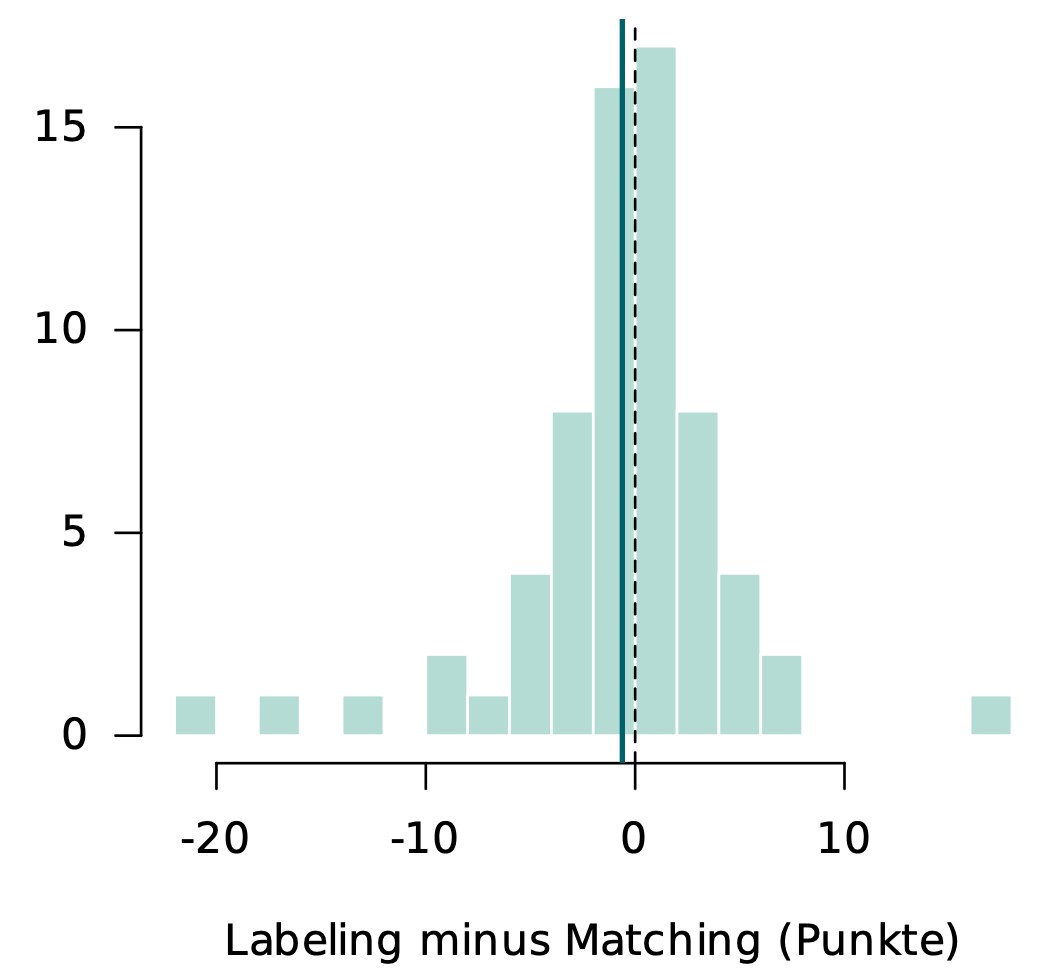
\includegraphics[width=\linewidth]{individuelle_differenzen.png}
 \caption{Craving nach Matching und Labeling bei 66 vollständigen Teilnahmen}
 \label{fig:testable-paired}
\end{figure}

Die Punktschätzung liegt zwar in der erwarteten Richtung eines geringeren Rauchverlangens nach Labeling, ist jedoch klein und mit null sowie mit geringfügig höherem Rauchverlangen vereinbar. Aus medizinisch-informatischer Sicht zeigt die Auswertung, dass die Rekonstruktion der Messbedingungen und die reproduzierbare Analyse mit einem zeitgemäßen, agilen Verfahren möglich sind.

\subsection{Reproduzierbarer R-Quelltext}
\label{sec:testable-r-code}
Listing~\ref{lst:testable-r} enthält den vollständigen ausführbaren Quelltext. Das Skript erzeugt aggregierte CSV-Ergebnisse, eine Vektorabbildung und die direkt eingebundenen LaTeX-Zahlen.

\lstinputlisting[language=R,basicstyle=\ttfamily\scriptsize,
 numbers=left,numberstyle=\tiny,numbersep=6pt,stepnumber=1,
 breaklines=true,breakatwhitespace=false,columns=fullflexible,
 keepspaces=true,showstringspaces=false,frame=single,
 caption={Vollständige R-Auswertung der Testable-Exporte},label={lst:testable-r}]
 {../analysis/testable/analyse_testable.R}

\begin{thebibliography}{1}
\bibitem{tabibnia_cuelabeling_2026} Tabibnia et al.:
Cue labeling reduces cigarette craving and associated neural activity.
Neuropsychopharmacology 51 (2026), 822--830.
\end{thebibliography}
\end{document}
